\chapter{Infinite dimensional preparation uncertainty}\label{chap:infinite-prep-ur}
\section{Introduction}
A standard introductory course on quantum mechanics, for example one following ref.~\cite{griffiths2005introduction},~\cite{Zettili} or~\cite{Shankar}, mentions several infinite dimensional state-spaces. Namely the pure states of a particle free to move on an line ($L^2(\R)$), a particle fixed to a one dimensional ring ($L^2(\circleNotate)$, where $\circleNotate$ denotes the unit circle), and a particle in a ``box'', a finite interval (without loss of generality $L^2([-\pi, \pi])$). Preparation uncertainty for position and momentum observables has been studied for several of these spaces, with the variance~\cite{Heisenberg1927-Wheeler+Zurek} and Shannon-entropy~\cites{Bialynicki-BirulaMycielski1975}{beckner-1975} uncertainty regions for the Euclidean spaces being characterised in 1927 and 1975, respectively. More recently the case of the particle on a ring has been addressed for both measurement uncertainty and preparation uncertainty~\cite{sharp-ur-num-angle}. 

There does not seem to have been a similar analysis for the particle in a box system. In part this omission may be due to the lack of phase-space symmetry which makes the problem more tractable in other cases. We contrast our approach with that taken in ref.~\cite{entropic-ur-infinite-well} which seems superficially similar, however the authors of that reference only examine the uncertainty of eigenstates of the Hamiltonian of the ``box'' system, rather than the full state-space. Our approach is more similar to the original Heisenberg result, in that we seek an uncertainty relation which is valid for all quantum states of the system.

We will be interested in comparing our results to those obtained for the ring, as well as the free particle. A barrier to this is that it is not possible to directly define the variance for a probability distribution defined on a circle. This may be seen by noting that in order to define the variance one must first define the mean and that, for example, the uniform distribution on the circle does not have a well-defined mean. For this reason Busch, Kiukas and Werner employed the  $\alpha$-deviation (see equation~\eqref{eqn:wassersten-variance}), in order to compare the localisation of probability distributions. 

In section~\ref{sec:box-ur-state-space} we will define the observables of interest, which will be obtained as restrictions of the standard position and momentum observables on $L^2(\R)$. We will also determine the relevant domain, the largest subspace of $L^2([-\pi,\pi])$ for which the first and second moments of both observables are finite. In section~\ref{sec:box-ur-structure} we will determine some constraints on the structure of the uncertainty region, in particular we show that it is the epigraph of a continuous function, which decreases on the interval $\left(0,\frac{\pi^2}{3}-2\right)$, attains a minimum of $\frac{1}{4}$ at $\frac{\pi^2}{3}-2$ and increases again on $\left(\frac{\pi^2}{3}-2, \pi^2\right)$. In addition the boundary function is convex in the interval on which it is increasing. In section~\ref{sec:box-ur-analytical-bounds} we obtain some analytical bounds on the boundary function, in particular showing it is bounded below by, and is asymptotic to, the hyperbola which bounds the free particle uncertainty region. In section~\ref{sec:box-ur-numerics} we discuss numerical approximations to the boundary curve, in particular we give a method to approximate a curve which upper bounds the boundary function. We prove that the curve which is being approximated is exactly the boundary function in the region where the latter is convex, and conjecture that this is also true outside this interval. Finally in section~\ref{sec:box-ur-comparisons} we compare the results for the box system with those already known for the particle on a ring, and the free particle. We note that the variance for the box system is the same as the $2$-deviation used for the analysis of the ring system in~\cite{sharp-ur-num-angle}, so it is reasonable to compare the two.

\section{State-space}\label{sec:box-ur-state-space}
We model the box system as one obtained from the full Hilbert space $L^2(\R)$ by imposing the restriction that the states are zero outside the interval $[-\pi, \pi]$, this is an idealisation of the physical situation where there are large (but finite) potential ``walls'' causing the probability density of the particle to decay rapidly outside the box. There is an obvious isometry $l:~L^2([-\pi,\pi])\to L^2(\R)$ which extends a state by $0$ outside the allowed interval
\begin{align}
  (l\varphi)(x) = \begin{cases}\varphi(x), &x\in [-\pi,\pi]\\ 0, &\text{otherwise}\end{cases},
\end{align}
from which we obtain position and momentum observables 
\begin{align}
  \ope:X &\mapsto l^* \ope_0(X) l\\
  \opf:Y &\mapsto l^* \opf_0(Y) l,
\end{align}
where $\ope$, $\ope$ are the observables (POVMs) acting on $L^2([-\pi,\pi])$ and $\ope_0$, $\opf_0$ are those for $L^2(\R)$, i.e. $\ope_0$, $\opf_0$ are the spectral measures of the standard position and momentum self-adjoint operators respectively. More explicitly $\ope_0(X)$ is the operator which multiplies by the characteristic function of the (Borel) set $X$, while $\opf_0$ is the Fourier transform
\begin{align}
  (\ope_0(X)\varphi)(x) &= \begin{cases}\varphi(x), &x\in X\\ 0, &\text{otherwise}\end{cases}\\
  (\opf_0(Y)\varphi)(x) &= (\fcal^*\ope_0(Y)\fcal)(x),
\end{align}
where the unitary $\fcal$ implements the Fourier transform
\begin{align}
  (\fcal\varphi)(p) &= \int_\R e^{-2\pi i x p} \varphi(x)dx.
\end{align}
We restrict our attention to those states for which the first and second moments of both observables are finite, this imposes some non-trivial conditions on the quantum states. 
\begin{thm}
  The first and second moments 
  \begin{align}
    \expe{\ope[1]}{\varphi} &= \int_\R x \braket{\varphi}{\ope(dx)\varphi} & \expe{\opf[1]}{\varphi} &= \int_\R p \braket{\varphi}{\opf(dp)\varphi}\\
    \expe{\ope[2]}{\varphi} &= \int_\R x^2 \braket{\varphi}{\ope(dx)\varphi} & \expe{\opf[2]}{\varphi} &= \int_\R p^2 \braket{\varphi}{\opf(dp)\varphi}. 
  \end{align}
  are finite on the domain of the self-adjoint operator
  \begin{align}\label{eqn:good-opf[2]-domain}
    \dom{\opf[1]^*\opf[1]} = \left\{\varphi\in\dom{\opf[1]}\,\middle|\,\varphi^{\prime} \text{ is abs. cont.},\,\varphi^{\prime\prime}\in L^2([-\pi,\pi])\right\},
  \end{align}
  furthermore they are not finite on any larger domain.
\end{thm}
\begin{proof}
The actions of the moments are exactly those of the more familiar operators on $L^2(\R)$, since they are just restrictions of those operators to $L^2([-\pi,\pi])$, so
\begin{align}
  \left(\ope[1]\varphi\right)(x) &= x\varphi(x) & \left(\opf[1]\varphi\right)(x) &= -i\varphi^\prime(x)\\
  \left(\ope[2]\varphi\right)(x) &= x^2\varphi(x) & \left(\opf[2]\varphi\right)(x) &= -\varphi^{\prime\prime}(x). 
\end{align}
The states $\varphi$ must be absolutely continuous, as well as taking the value $0$ at the boundary points, $-\pi$ and $\pi$, in order that $l\varphi$ is in the domain of $\opf_0[1]$. We note that $\opf[1]$ is \emph{not} a self-adjoint operator on its domain,
\begin{align}
  \dom{\opf[1]} = \left\{\varphi\in L^2([-\pi,\pi])\, \middle|\, \varphi \text{ is abs. cont., } \varphi^\prime\in L^2([-\pi,\pi]),\, \varphi(-\pi) = \varphi(\pi) = 0\right\},
\end{align}
and therefore the expectation of the second moment $\opf[2]$ is finite on a larger set than 
\begin{align}\label{eqn:bad-opf[2]-domain}
  \dom{\opf[1]\opf[1]} = \left\{\varphi\in\dom{\opf[1]}\,\middle|\,\left(\opf[1]\varphi\right)\in\dom{\opf[1]}\right\}.
\end{align}
The difference between equations \eqref{eqn:bad-opf[2]-domain} and \eqref{eqn:good-opf[2]-domain} being that in the latter we have the extra condition that $\varphi^\prime(-\pi) = \varphi^\prime(\pi) = 0$. To prove that this is the largest possible domain for $\opf[2]$ we recall that the integral of a real function against a POVM is a symmetric operator (see, e.g., \cite{quantum-measurement-busch-et-al}, chapter 4) and that von Neumann's formulas imply that a densely defined self adjoint operator can have no proper symmetric extensions. Indeed any symmetric extension of a densely defined symmetric operator $\opa$ is a restriction of $\opa^*$~\cite{akhiezer-glazman-lin-ops-hilb-space}.

It remains to show that the domain of $\opf[1]^*\opf[1]$ is indeed the set given in \eqref{eqn:good-opf[2]-domain}, which we may verify using integration by parts, recalling that the domain of $\opf[1]^*$ is given by the set of vectors $\psi$ such that there exists a vector $\xi\in L^2([-\pi,\pi])$ such that for all $\phi\in\dom{\opf[1]}$
\begin{align}
  \braket{\psi}{\opf[1]\phi} = \braket{\xi}{\phi}.
\end{align}
In the position representation we therefore have
\begin{align}
  \braket{\psi}{\opf[1]\phi} &= \braket{\xi}{\phi}\\
  \int_{-\pi}^{\pi}dx\psi(x)^*(-i)\phi^\prime(x) &= \int_{-\pi}^{\pi}dx \xi(x)^* \phi(x), \\
                             &= \left.\Xi(x)\phi(x)\right\vert_{-\pi}^{\pi} + \int_{-\pi}^{\pi}dx i\Xi(x)^* \phi^\prime(x)\\
                             &= \int_{-\pi}^{\pi}dx i\Xi(x)^* \phi^\prime(x), 
\end{align}
where
\begin{align}
  \Xi(x) = \xi(-\pi)+\int_{-\pi}^{x}dy\xi(y),
\end{align}
exists since we assume $\xi\in L^2([-\pi,\pi])$ and the interval is bounded, while $\phi^\prime$ exists since we are assuming $\phi\in\dom{\opf[1]}$. A standard argument, choosing $\phi$ such that $\phi^\prime$ ranges over a basis for~$L^2([-\pi,\pi])$ now ensures that
\begin{align}
  \psi(x) &= -i\Xi(x)\\
          &= -i\xi(-\pi)-i\int_{-\pi}^{x}dy\xi(y).
\end{align}
There therefore exists a Lebesgue integrable function $g$ such that 
\begin{align}
  \psi(x) = \psi(-\pi) + \int_{-\pi}^xdy g(y),
\end{align}
by Lebesgue's fundamental theorem of calculus this is equivalent to $\psi$ being absolutely continuous.

We do not require any additional conditions to ensure that the moments of position are finite, since absolute continuity, combined with the boundary conditions, implies that the states are bounded functions in the position representation.
\end{proof}

Due to the boundary conditions in \eqref{eqn:good-opf[2]-domain} we do not have shift operators, which move the states in position space. Explicitly, given a pure state $\varphi\in\dom{\opf[1]^*\opf[1]}$, and $a\in [0,2\pi] $ the function
\begin{align}
  \tilde{\varphi}&:[-\pi,\pi]\to \Cx\\
  \tilde{\varphi}&:x\mapsto \begin{cases}\varphi(x+a), & x+a\in [-\pi,\pi]\\ \varphi(x+a-2\pi), & x+a-2\pi\in [-\pi,\pi]\end{cases},
\end{align}
will generally \emph{not} obey the boundary conditions and therefore will not be a state. This ability to shift states is a key point in proofs of the usual Heisenberg uncertainty relation for the particle on the line. In particular on the real line one can shift any state in order to set the expectation values of position and momentum to zero, at which point the variance functional becomes linear in the state, offering a significant simplification.

We do, however, have the ability to shift the expectation of the first moment of momentum of the states as we choose. 
\begin{lem}\label{lem:infinite-dim-ur-shift-momentum}
  Given $\varphi\in\dom{\opf[1]^*\opf[1]}$ and $a\in\R$ there exists $\varphi_a\in\dom{\opf[1]^*\opf[1]}$ such that
  \begin{align}
    \expe{\ope[1]}{\varphi_a} &= \expe{\ope[1]}{\varphi} & \expe{\opf[1]}{\varphi_a} &= \expe{\opf[1]}{\varphi} + a\\
    \expe{\ope[2]}{\varphi_a} &= \expe{\ope[2]}{\varphi}& \expe{\opf[2]}{\varphi_a} &= \expe{\opf[2]}{\varphi} + 2a\expe{\opf[1]}{\varphi} + a^2.
  \end{align}
  Further, these formulae imply that
  \begin{align}
    \var[\varphi_a]{\ope} &= \var[\varphi]{\ope}\\
    \var[\varphi_a]{\opf} &= \var[\varphi]{\opf}.
  \end{align}
\end{lem}
\begin{proof}
Given $\varphi\in\dom{\opf[1]^*\opf[1]}$ and $a\in\R$ the map
\begin{align}
  M_a &:\dom{\opf[1]^*\opf[1]}\to\dom{\opf[1]^*\opf[1]}\\
  (M_a\varphi)&:x\mapsto e^{i a x}\varphi(x),
\end{align}
leaves the variance of momentum unchanged, along with the expectation of all the moments of position. As required $M_a$ changes the expectation of the first moment of momentum by $a$
\begin{align}
  \expe{\ope[1]}{M_a\varphi} &= \expe{\ope[1]}{\varphi} & \expe{\opf[1]}{M_a\varphi} &= \expe{\opf[1]}{\varphi} + a\\
  \expe{\ope[2]}{M_a\varphi} &= \expe{\ope[2]}{\varphi}& \expe{\opf[2]}{M_a\varphi} &= \expe{\opf[2]}{\varphi} + 2a\expe{\opf[1]}{\varphi} + a^2.
\end{align}
These formulae may be proved by expressing the states in the position representation and computing
\begin{align}
  (\ope[1]M_a\varphi)(x) &= -i \frac{d}{dx}\left(e^{iax}\varphi(x)\right)\\
                         &= e^{iax}\left(a\varphi(x) -i\varphi^\prime(x)\right),
\end{align}
and
\begin{align}
  (\ope[2]M_a\varphi)(x) &= - \frac{d^2}{dx^2}\left(e^{iax}\varphi(x)\right)\\
                         &= -i\frac{d}{dx} e^{iax}\left(a\varphi(x) -i\varphi^\prime(x)\right)\\
                         &= e^{iax}\left(a^2\varphi(x) -2 a i\varphi^\prime(x)- \varphi^{\prime\prime}(x)\right),
\end{align}
before computing the integrals that form the inner products.
\end{proof}
% To prove this we first note that since $\varphi$ is a (normalised) state, $\ope_0$ a projection-valued measure, $l$ an isometry and $\fcal$ a unitary we have that 
% \begin{align}\label{eqn:interferometric-ur-measure-bounded-by-1}
%   0\leq\int_P \braket{\varphi}{\opf(dp)\varphi} \leq \int_P dp,
% \end{align}
% for all measurable sets $P$. In particular this implies
% \begin{align}
%    \abs{\int_{-1}^1 p^k \braket{\varphi}{\opf(dp)\varphi} } \leq 2.
% \end{align}
% We split the integral defining the second moment into three parts
% \begin{align}
%   \expe{\opf[2]}{\varphi} &= \int_\R p^2 \braket{\varphi}{\opf(dp)\varphi}\\
%                           &= \int_{-\infty}^{-1} p^2 \braket{\varphi}{\opf(dp)\varphi} + \int_{-1}^{1} p^2 \braket{\varphi}{\opf(dp)\varphi} + \int_1^{\infty} p^2 \braket{\varphi}{\opf(dp)\varphi},
% \end{align}
% and note the inequalities
% \begin{align}
%   0&\leq - \int_{-\infty}^{-1} p \braket{\varphi}{\opf(dp)\varphi}  \leq \int_{-\infty}^{-1} p^2 \braket{\varphi}{\opf(dp)\varphi}\\
%   0&\leq  \int_1^{\infty} p \braket{\varphi}{\opf(dp)\varphi}  \leq \int_1^{\infty} p^2 \braket{\varphi}{\opf(dp)\varphi}.
% \end{align}
% Combining these with the fact that equation \eqref{eqn:interferometric-ur-measure-bounded-by-1} implies that
% \begin{align}
%   \int_{-1}^{1} p \braket{\varphi}{\opf(dp)\varphi} < 2
% \end{align}


% note that $\opf[1]^*\opf[1]$ is self-adjoint (indeed it is positive) on it's domain. Its action, when expressed in the position representation, is
% \begin{align}
%   (\opf[1]^*\opf[1]\varphi)(x) = -\varphi^{\prime\prime}(x).
% \end{align}

\section{Structure of the uncertainty region}\label{sec:box-ur-structure}

We are interested in the region
\begin{align}
  U = \left\{(\varr{\ope}, \varr{\opf}))\middle|\rho\in \dops\right\},
\end{align}
where $\dops$ is the set of density operators over the $\dom{\opf[1]^*\opf[1]}$, that is the set of operators of the form
\begin{align}
  \sum_k p_k P_k,
\end{align}
such that the $P_k$ are mutually orthogonal projectors onto subspaces of $\dom{\opf[1]^*\opf[1]}$, $p_k\geq 0$ and
\begin{align}
  \sum_k p_k = 1.
\end{align}

For convenience we summarise the results of this section in proposition~\ref{prop:box-ur-structure-summarise-prop}.
\begin{prop}\label{prop:box-ur-structure-summarise-prop}
  The uncertainty region $U$ is the epigraph of a function $b:(0,\pi^2)\to \R$. Further
  \begin{enumerate}
    \item $b$ is continuous.
    \item $b$ has a global minimum $b(x)\geq b\left(\frac{\pi^2}{3} -2\right) = \frac{1}{4}$.
    \item The minimum is unique.
    \item The minimum is achieved by the state $\psi_0:x\mapsto \frac{1}{\sqrt{\pi}}\sin\left(\frac{1}{2}(x-\pi)\right)$.
    \item $b$ is decreasing on $\left(0,  \frac{\pi^2}{3} -2\right)$ and increasing on $\left(\frac{\pi^2}{3} -2, \pi^2\right)$.
    \item $b$ is convex on the interval $\left(\frac{\pi^2}{3} -2, \pi^2\right)$.
  \end{enumerate}
\end{prop}

It is clear that the region is contained in the quadrant with $0 \leq\var[\rho]{\ope}$, $0\leq\var[\rho]{\opp}$, further, since the interval is bounded above and below by $\pi$ and $-\pi$, we must have that $\var[\rho]{\ope} \leq \expe{\ope[2]}{\rho} \leq \pi^2$. These bounds are classical, for example the probability distribution which assigns probability $\frac{1}{2}$ to each of the points $-\pi$ and $\pi$ has (classical) position variance $\pi^2$.

\begin{lem}\label{lem:box-ur-all-points-filled}
  For any $x\in (0, \pi^2)$ there exists a state $\varphi\in\dom{\opf[1]^*\opf[1]}$  such that 
  \begin{align}
    \var[\varphi]{\ope} = x.
  \end{align}
\end{lem}
\begin{proof}
Take any smooth, $L^2$ normalised, function $f: \mathbb{R} \to \mathbb{R}$, supported only on $[0,1]$, and consider
\begin{equation}
	g_{a,s}(x) = \frac{1}{\sqrt{2s}}f\left(\frac{x-a}{s}\right) +\frac{1}{\sqrt{2s}}f\left(\frac{-x-a}{s}\right),
\end{equation}
where a is non-negative, s is positive and they are taken such that $a+s < \pi$. The resulting $g_{a,s}$ is a smooth function supported on $[-a-s, -a] \cup [a,a+s]$, with $\expe{\opq}{g_{a,s}} = 0$, and so has finite momentum variance as well as
\begin{equation}
	a^2 < \var{\opq}{g_{a,s}} < (a+s)^2.
\end{equation}
By varying $a$ and $s$ in the allowed region we see that in any interval $I = (\alpha, \alpha+\varepsilon) \subset (0,\pi^2)$ there exists some state $\varphi$ with $\var[\varphi]{\ope} \in I$. Further, given any two position uncertainties $\var[\varphi]{\ope}$ and $\var[\psi]{\opq}$, achieved by pure states $\varphi$ and $\psi$ we can define the state
\begin{align}
	\xi_\theta &= \frac{1}{\sqrt{1+2\cos\theta\sin\theta\Re\left(\braket{\varphi}{\psi}\right)}}\left(\cos\theta\,\varphi + \sin\theta\,\psi \right),
\end{align}
and the continuous, real valued function $\theta\mapsto\var[\xi_\theta]{\opq}$. The intermediate value theorem then asserts that for every variance $v\in(\var[\varphi]{\opq},\var[\psi]{\opq})$ there exists $\theta^*\in(0,\pi)$ such that $\var[\xi_{\theta^*}]{\opq} = v$.
\end{proof}

\begin{lem}\label{lem:box-ur-half-line-contained}
Given a state $\varphi$ with variances $(\var[\varphi]{\ope}, \var[\varphi]{\opf})$ the half-line
\begin{align}
  L = \left\{(\var[\varphi]{\ope}, y)\middle| y \geq \var[\varphi]{\opf}\right\},
\end{align}
is contained in the uncertainty region.
\end{lem}
\begin{proof}
We apply the map 
\begin{align}
  M_a : \varphi &\mapsto \left(x \mapsto \varphi(x) e^{a i x^2}\right),
\end{align}
to obtain a new state, for which the expectations and variances can be computed
\begin{align}
  \expe{\ope[1]}{M_a\varphi}&= \expe{\ope[1]}{\varphi} & \expe{\opf[1]}{M_a\varphi} &= \expe{\opf[1]}{\varphi} + 2a\expe{\ope[1]}{\varphi}\\
  \expe{\ope[2]}{M_a\varphi}&= \expe{\ope[2]}{\varphi} & \expe{\opf[2]}{M_a\varphi} &= \expe{\opf[2]}{\varphi} + 4a^2\expe{\ope[2]}{\varphi}\\
  \var[M_a\varphi]{\ope} &= \var[\varphi]{\ope} & \var[M_a\varphi]{\opf} &= \var[\varphi]{\opf} + 4 a^2 \var[\varphi]{\ope} - 2a\expe{\ope[1]}{\varphi}\expe{\opf[1]}{\varphi}.
\end{align}
Since $0<\var[\varphi]{\ope}$ for all states $\varphi$ there exists an $a$ such that $\var[M_a\varphi]{\opf} = y$, for all $y \geq \var[\varphi]{\opf}$.
\end{proof}

This offers a convenient description of the uncertainty region in terms of a boundary function.
\begin{lem}
  The uncertainty region is the epigraph (the set of points lying above the graph) of the function
  \begin{align}
    b&:(0,\pi^2) \to \R\\
    b&:x\mapsto \inf\left\{\var[\varphi]{\opf}\,\middle|\,\var[\varphi]{\ope} = x\right\}.\label{eqn:box-ur-boundry-func-defn}
  \end{align}
\end{lem}
Loosely this means that in addition to being unbounded above the uncertainty region has no ``holes'' in it.
\begin{proof}
  In order to define such a function it is necessary that for each $x\in (0,\pi^2)$ the infimum in equation~\eqref{eqn:box-ur-boundry-func-defn} exists and is finite. This is true since the set the infimum is being taken over is non-empty (by lemma~\ref{lem:box-ur-all-points-filled}) and bounded below (by $0$, since the variance is non-negative). 

The uncertainty region $U$ contains the epigraph of $b$ if all the points above $b$ are in $U$, which follows from lemma~\ref{lem:box-ur-half-line-contained} combined with the definition of $b$. If $(x,y)$ is a point not in $U$ then there is no point directly below\footnote{By directly below (resp. above) $(x,y)$ we here mean a point $(x,y^\prime)$ such that $y^\prime < y$ (resp. $y^\prime > y$).} $(x,y)$ which is in $U$ due to lemma~\ref{lem:box-ur-half-line-contained}, therefore $y$ is a lower bound for the set
\begin{align}
  U(x) = \left\{\var[\varphi]{\opf}\,\middle|\,\var[\varphi]{\ope} = x\right\}.
\end{align}
From the definition of $b(x)$ have $y \leq b(x)$, since $y$ is a lower bound for $U(x)$ and $b(x)$ is the greatest lower bound for $U(x)$, so $(x,y)$ is not in the epigraph of $b$. 

Conversely the epigraph of $b$ contains $U$, which can be seen by noting that for each $x\in (0,\pi^2)$, all of the points $(x,y)$ in the uncertainty region are, by definition directly above $b(x)$.
\end{proof}
We can find the minimum of $b$. 
\begin{lem}
  For all $x\in (0,\pi^2)$
  \begin{align}
    b\left(\frac{\pi^2}{3} - 2\right) = \frac{1}{4} \leq b(x).
  \end{align}
  Further this minimum is achieved by the state
  \begin{align}
     \psi_0 = \frac{1}{\sqrt{\pi}}\sin\left(\frac{1}{2}(x-\pi)\right),
  \end{align}
  and is unique
  \begin{align}
    x\neq\frac{\pi^2}{3} - 2 \implies \frac{1}{4} < b(x).
  \end{align}
\end{lem}
\begin{proof}
We first seek the least eigenvalue of the self-adjoint operator $\opf[2] = \opf[1]^*\opf[1]$. It is well known that the solutions to
\begin{align}
  -\varphi^{\prime\prime} = \lambda\varphi
\end{align}
are sines and cosines. Applying the boundary conditions $\varphi(-\pi)=\varphi(\pi)=0$ implies that the eigenstates are
\begin{align}
  \psi_k(x) = \frac{1}{\sqrt{\pi}}\sin\left(\frac{k+1}{2}(x-\pi)\right), \qquad k\in\{0,1,2,\hdots\}
\end{align}
and the eigenvalues are
\begin{align}
  \opf[2]\psi_k(x) = \frac{(k+1)^2}{4}\psi_k(x),
\end{align}
where we have chosen the form such that $\psi_k$ is an odd function if $k$ is odd, and even if $k$ is even. Note that each eigenspace is one-dimensional, in particular there is only one state (up to phase) attaining the value $\expe{\opf[2]}{\psi_0} = \frac{1}{4}$. One can compute
\begin{align}
  \expe{\opf[1]}{\psi_k} &= -i\int_{-\pi}^\pi dx \psi_k(x)^* \psi_k^\prime(x)\\
                         &= -i\frac{k+1}{2\pi}\int_{-\pi}^\pi dx \sin\left(\frac{k+1}{2}(x-\pi)\right) \cos\left(\frac{k+1}{2}(x-\pi)\right)\\
                         &= 0,
\end{align}
so applying lemma~\ref{lem:infinite-dim-ur-shift-momentum} the least eigenvalue of $\opf[2]$ is exactly the least possible momentum variance,
\begin{align}
  \inf\left\{\varr{\opf}\,\middle|\,\rho\in\dom{\opf[2]}\right\} = \frac{1}{4}.
\end{align}
We also compute the position variance of the state $\psi_0$ which minimises the momentum variance
\begin{align}
  \var[\psi_0]{\ope} &= \expe{\ope[2]}{\psi_0} - \expe{\ope[1]}{\psi_0}^2\\
                     &= \frac{1}{\pi}\int_{-\pi}^\pi dx x^2 \sin\left(\frac{1}{2}(x-\pi)\right)^2 - \left(\frac{1}{\pi}\int_{-\pi}^\pi dx x \sin\left(\frac{1}{2}(x-\pi)\right)^2\right)^2\\
                     &= \frac{\pi^2}{3} - 2.
\end{align}
Finally we show the minimum is unique. Assume a state achieves 
\begin{align}
  \var[\varphi]{\opf} = \frac{1}{4},
\end{align}
then we can employ lemma~\ref{lem:infinite-dim-ur-shift-momentum} to obtain a state $\xi$ with
\begin{align}
  \expe{\opf[1]}{\xi} = 0\\
  \expe{\opf[2]}{\xi} = \frac{1}{4},
\end{align}
the fact that the eigenspaces of $\opf[2]$ are one dimensional then implies that 
\begin{align}
  \xi = \alpha \psi_0,
\end{align}
for some complex phase $\alpha$. Reversing the transformation from the proof of lemma~\ref{lem:infinite-dim-ur-shift-momentum} then implies that
\begin{align}
  \varphi(x) = \alpha e^{-iax}\psi_0(x),
\end{align}
for some $a\in\R$. It follows that 
\begin{align}
  \var[\varphi]{\opf} = \var[\psi_0]{\opf} = \frac{\pi^2}{3}-2,
\end{align}
and so the minimum of $b$ is unique.
\end{proof}

The minimum splits $b$ into two regions, to the left of the minimum $b$ is decreasing and to the right it is increasing.
\begin{lem}\label{lem:box-ur-fn-dec-inc}
  The boundary function $b$ is strictly decreasing on $\left(0, \frac{\pi^2}{3}-2\right)$ and strictly increasing on $\left(\frac{\pi^2}{3}-2, \pi^2\right)$.
\end{lem}
\begin{proof}
  Choose $x,y \in \left(0,\frac{\pi^2}{3}-2\right)$, without loss of generality let $x < y$, and choose a sequence of states $\rho_n$ such that
  \begin{align}%n > m &\implies \var[\rho_n]{\opf} < \var[\rho_m]{\opf}\\
    \var[\rho_n]{\ope} &= x\\
    \lim_{n\to\infty}\var[\rho_n]{\opf} &=b(x).
  \end{align}
  Such a sequence exists due to the definition of $b(x)$. Without loss of generality, due to lemma~\ref{lem:infinite-dim-ur-shift-momentum} choose
  \begin{align}
    \expe{\opf[1]}{\rho_n} = 0.
  \end{align}
  Now we mix these states with the projector onto the minimizer of the momentum variance, $\ketbra{\psi_0}{\psi_0}$, and define the functions
  \begin{align}
    f_n&:(0,1) \to \R\\
    f_n&:\lambda \to \var[\lambda\rho_n+(1-\lambda)\ketbra{\psi_0}{\psi_0}]{\ope},
  \end{align}
  by continuity, for each $n\in\N$ there exists $\lambda^*\in (0,1)$ such that $f_n(\lambda) = y$. Now by the definition of $b$ we have
  \begin{align}
    b(y) &\leq \expe{\opf[2]}{\lambda^*\rho_n+(1-\lambda^*)\ketbra{\psi_0}{\psi_0}}\\
         &= \lambda^*\expe{\opf[2]}{\rho_n}+(1-\lambda^*)\expe{\opf[2]}{\ketbra{\psi_0}{\psi_0}}\\
         &< \expe{\opf[2]}{\rho_n}.
  \end{align}
  Taking the limit $n\to\infty$ of the last inequality gives
  \begin{align}
    b(y) \leq b(x),
  \end{align}
  as required. The proof for the increasing region is essentially identical.
\end{proof}

We recall that the variance is concave as a function of the (mixed) state.
\begin{lem}\label{lem:box-ur-variance-concave}
  Given any observable $\opa$, if $\dops$ is the set of density operators for which the first and second moments of $\opa$ are finite then the map $\nu:\dops\to \R$, $\nu:\rho\mapsto \varr{\opa}$ is concave.
\end{lem}
\begin{proof}
  Take $\rho,\, \sigma \in \dops$ with finite first and second moments of $\opa$ and choose $\lambda \in (0,1)$ then
  \begin{align}
    0&\leq \lambda(1-\lambda) \left(\expe{\opa}{\rho} - \expe{\opa}{\sigma}\right)^2\\
    \lambda^2 \expe{\opa}{\rho}^2 + (1- \lambda)^2\expe{\opa}{\sigma}^2 + 2\lambda(1-\lambda)\expe{\opa}{\rho}\expe{\opa}{\sigma} &\leq \lambda \expe{\opa}{\rho}^2 + (1-\lambda) \expe{\opa}{\sigma}^2\\
    \left(\lambda \expe{\opa}{\rho} + (1- \lambda)\expe{\opa}{\sigma}\right)^2 &=\\
    \expe{\opa^2}{\lambda\rho + (1-\lambda)\sigma} - \left(\lambda \expe{\opa}{\rho} + (1- \lambda)\expe{\opa}{\sigma}\right)^2 &\geq \lambda\left(\expe{\opa^2}{\rho} -\expe{\opa}{\rho}^2\right) + (1-\lambda)\left(\expe{\opa}{\sigma}^2 -\expe{\opa}{\sigma}^2\right)\\
    \var[\lambda\rho + (1-\lambda)\sigma]{\opa} &\geq \lambda \var{\opa}{\rho} + (1-\lambda) \var{\opa}{\sigma}.
  \end{align}
\end{proof}
\begin{lem}\label{lem:increasing-line-segments-contained}
  If $(v,w), (x,y)\in U$ and $v<x$, and $w < y$ then 
  \begin{align}
    \lambda(v,w) + (1-\lambda)(x,y)\in U,
  \end{align}
  for all $\lambda\in (0,1)$.
\end{lem}
\begin{proof}
  We choose density operators $\rho,\sigma$ such that
  \begin{align}
    \var[\rho]{\ope} &= v & \var[\sigma]{\ope} &= x \\
    \var[\rho]{\opf} &= w & \var[\sigma]{\opf} &= y \\
    \expe{\opf[1]}{\rho} &= 0 & \expe{\opf[1]}{\sigma} &= 0,
  \end{align}
  Consider the real, continuous function
  \begin{align}
    f:\lambda \mapsto \var[\lambda\rho+ (1-\lambda)\sigma]{\ope}.
  \end{align} 
  By continuity, for any $\lambda\in (0,1)$ there exists $\mu\in (0,1)$ such that
  \begin{align}
    f(\mu) = \lambda v + (1-\lambda)x.
  \end{align}
  Due to the concavity of the variance functional (lemma~\ref{lem:box-ur-variance-concave}) $f$ is concave and 
  \begin{align}
    f(\mu) &\geq \mu v + (1-\mu)x\\
    \lambda v + (1-\lambda)x &\geq \mu v + (1-\mu)x\\
    \lambda (v-x) &\geq \mu(v-x)\\
    \implies \lambda &\leq \mu.
  \end{align}
  Then $w < y$ implies
  \begin{align}
    \mu w + (1-\mu) y \leq \lambda w + (1-\lambda)y.
  \end{align}
  Since we chose $\rho$ and $\sigma$ such that the first moments of momentum are zero, the momentum variance is linear in the state and
  \begin{align}
    \var[\mu\rho+ (1-\mu)\sigma]{\ope} &= \mu w + (1-\mu) y\\
                                           &\leq \lambda w + (1-\lambda)y.
  \end{align}
  Recall we are attempting to show that the point $\lambda(v,w) + (1-\lambda)(x,y)\in U$, but we have now shown that the point $(\lambda v + (1-\lambda) x, \mu w + (1-\mu) y)\in U$, and $\mu w + (1-\mu) y < \lambda w + (1-\lambda)y$. We can now employ lemma~\ref{lem:box-ur-half-line-contained} to move directly up in the uncertainty region to get to the desired point.
\end{proof}

\begin{lem}
The boundary function $b$ is convex on $\left(\frac{\pi^2}{3}-2, \pi^2\right)$.
\end{lem}
\begin{proof}
  The boundary function $b$ is convex on this interval iff the restriction of the uncertainty region
  \begin{align}
    U_{>} = \left\{(x,y)\in U\,\middle|\,x >\frac{\pi^2}{3}-2 \right\},
  \end{align}
  is convex. We therefore have to show that for any two points $(v,w), (x,y)\in U_{>}$ the points
  \begin{align}
    \lambda(v,w) + (1-\lambda)(x,y)\in U,
  \end{align}
  for all $\lambda\in (0,1)$. Without loss of generality we choose $v < x$, we wish to employ lemma~\ref{lem:increasing-line-segments-contained} but we do not necessarily have $w < y$. We therefore consider a new point $(v,w^\prime)\in U_{>}$, directly below $(v,w)$. Since we have shown in lemma~\ref{lem:box-ur-fn-dec-inc} that the boundary curve is increasing in this interval we can choose $w^\prime \leq y$. By lemma~\ref{lem:increasing-line-segments-contained} we have that 
\begin{align}
  \lambda (v,w^\prime) + (1-\lambda)(x,y)\in U.
\end{align}
Employing lemma~\ref{lem:box-ur-half-line-contained} and noting that $w^\prime < w\implies \lambda w^\prime + (1-\lambda) y < \lambda  w+ (1-\lambda) y$ proves that $\lambda  w+ (1-\lambda) y$ is in the uncertainty region as required.
\end{proof}

A useful feature of the particle on a line is the ability to rescale states, if $\varphi\in L^2(\R)$, and $a > 0$ then
\begin{align}
  \varphi_a:x\mapsto\sqrt{a}\varphi{ax},
\end{align}
is also a state. We do not have this symmetry in the particle in a box system, since ``broadening'' a state will generally break the boundary conditions, but we can ``squeeze'' states if we wish.
\begin{lem}\label{lem:box-ur-squeeze-states}
  If $\varphi\in\dom{\ope[2]}$, $a \geq 1$ and
  \begin{align}
    \varphi_a:x\mapsto\begin{cases}\sqrt{a}\varphi(ax),& \abs{ax}\leq \pi\\ 0, &\text{otherwise}\end{cases},
  \end{align}
  then $\varphi_a\in\dom{\ope[2]}$, further
  \begin{align}
    \var[\varphi_a]{\ope} &= \frac{1}{a^2}\var[\varphi]{\ope}\label{eqn:box-ur-rescaling-1}\\
    \var[\varphi_a]{\opf} &= a^2\var[\varphi]{\opf}.\label{eqn:box-ur-rescaling-2}
  \end{align}
\end{lem}
\begin{proof}
  It is well known that this rescaling preserves the domains of the moments of the position and momentum observables on $L^2(\R)$. The only additional constraint in the present case is the imposition of the boundary conditions, which are easily shown to be preserved. One can verify equations~\eqref{eqn:box-ur-rescaling-1} and~\eqref{eqn:box-ur-rescaling-2} by directly computing the integrals.
\end{proof}

\begin{lem}
  The boundary function $b$ is continuous.
\end{lem}
\begin{proof}
  Convex functions are continuous, so $b$ is automatically continuous on $\left(\frac{\pi^2}{3}-2, \pi^2\right)$. In order to show that $b$ is continuous on $\left(0, \frac{\pi^2}{3}-2\right)$ we recall that $b$ is decreasing in this interval (lemma~\ref{lem:box-ur-fn-dec-inc}), that monotone functions have limits from the left and the right at every point, and can only have jump discontinuities.

We assume that there exists some discontinuity at a point $a\in\left(0, \frac{\pi^2}{3}-2\right)$ so that
\begin{align}
  \lim_{x\to a^-}b(x) = \lim_{x\to a^+}b(x) + \alpha,
\end{align}
where monotonicity implies $\alpha > 0$. We choose a sequence of states $\rho_n$ such that
\begin{align}
  \lim_{n\to\infty}\var[\rho_n]{\ope} &= x\\
  \var[\rho_n]{\ope} &\geq a\\
  \lim_{n\to\infty}\var[\rho_n]{\opf} &= \lim_{x\to a^+}b(x).
\end{align}
We fix $y < a$ then apply the ``squeezing map'' from lemma~\ref{lem:box-ur-squeeze-states} to each $\rho_n$ to obtain a sequence of states $\sigma_n$ such that
\begin{align}
  \var[\sigma_n]{\ope} = y,
\end{align}
then 
\begin{align}
  \var[\sigma_n]{\ope}\var[\sigma_n]{\opf} &= \var[\rho_n]{\ope}\var[\rho_n]{\opf}\\
  y b(y) &\leq \var[\rho_n]{\ope}\var[\rho_n]{\opf},
\end{align}
since, by definition, $b(y)\leq \var[\sigma_n]{\opf}$. Taking the limit $n\to\infty$ on the right hand side then gives the second inequality of
\begin{align}
  y \lim_{x\to a^+}b(x) \leq y b(y) \leq a \lim_{x\to a^+}b(x),
\end{align}
where the first inequality is just the monotonicity of $b$. Now taking the limit $y\to a^-$ gives
\begin{align}
  a \lim_{x\to a^+}b(x) \leq a \lim_{y\to a^-}b(y) \leq a \lim_{x\to a^+}b(x),
\end{align}
so $\lim_{y\to a^-}b(y) = \lim_{x\to a^+}b(x)$ implying $\lim_{x\to a}b(x)$ exists. A simple generalisation (choosing $\sigma_n$ such that $\var[\sigma_n]{\ope} = a$) establishes that $\lim_{y\to a}b(y) = b(a)$.

It remains to show that $b$ is continuous at the point $a=\frac{\pi^2}{3}-2$. This can be achieved by slightly altering the proof of lemma~\ref{lem:box-ur-fn-dec-inc}. We fix $v < \frac{\pi^2}{3}-2$ and choose a state $\rho$ such that
\begin{align}
  \var[\rho]{\ope} &= v\\
  \expe{\opf[1]}{\rho} &= 0.
\end{align} 
Then consider the states
\begin{align}
  \sigma(\lambda) = \lambda\rho + (1-\lambda)\ketbra{\psi_0}{\psi_0}.
\end{align}
As before, for each $x\in \left(v,\frac{\pi^2}{3}-2\right)$ there exists some $\lambda(x)$ such that 
\begin{align}
  \var[\sigma(\lambda(x))]{\ope} &= x,
\end{align}
then, by construction
\begin{align}
  \frac{1}{4} \leq b(x) &\leq \var[\sigma(\lambda(x))]{\opf}\\
                        &= \lambda(x)\var[\rho]{\opf} + (1-\lambda(x))\var[\ketbra{\psi_0}{\psi_0}]{\opf}.
\end{align}
Now as $x\to a^-$ we have $\lambda\to 0^+$ and obtain
\begin{align}
  \frac{1}{4} \leq \lim_{x\to a^-} b(x) \leq \frac{1}{4}.
\end{align}
The proof for $x\to a^+$ is similar.
\end{proof}

\section{Analytical bounds on the boundary function}
\label{sec:box-ur-analytical-bounds}
We first note that a simple bound may be obtained by recalling that the position and momentum observables $\ope,\opf$ we have defined are essentially restrictions of the standard position and momentum observables on $L^2(\R)$. In particular given a state $\varphi\in\dom{\opf}$ there exists a state $(l\varphi)\in L^2(\R)$ such that
\begin{align}
  \expe{\ope[1]}{\varphi} &= \expe{\ope_0[1]}{l\varphi} & \expe{\ope[2]}{\varphi} &= \expe{\ope_0[2]}{l\varphi}\\
  \expe{\opf[1]}{\varphi} &= \expe{\opf_0[1]}{l\varphi} & \expe{\opf[2]}{\varphi} &= \expe{\opf_0[2]}{l\varphi},
\end{align}
where $\ope_0, \opf_0$ are the position and observables on $L^2(\R)$, respectively. This means that the lower bound
\begin{align}\label{eqn:box-ur-hesenberg-is-a-lower-bound}
  \var[\varphi]{\ope}\var[\varphi]{\opf} \geq \frac{1}{4},
\end{align}
due to Heisenberg, is still valid for the box system. We can not expect that the Heisenberg bound will be tight for the box, since it is saturated by Gaussian states and these certainly do not obey the boundary conditions $\varphi(-\pi) = \varphi(\pi) = 0$. We can compare this lower bound to upper bounds obtained by considering families of states in $\dom{\opf}$. An obvious family of states is achieved by squeezing the minimizer of momentum, to obtain the bounds
\begin{align}
  \frac{1}{4x}\leq b(x) \leq \frac{1}{4x}\left(\frac{\pi^2}{3}-2\right),
\end{align}
valid for $x\in\left(0, \frac{\pi^2}{3}-2\right)$. 

\begin{lem}\label{lem:box-ur-b-asymptotic-to-hyperbola}
  As the position variance becomes small the boundary function $b$ is asymptotic to the canonical hyperbola, that is
  \begin{align}
    \lim_{x\to 0} x b(x) = \frac{1}{4}.
  \end{align}
\end{lem}
\begin{proof}
An upper bound for $b$, may be computed using the family of ``tempered-Gaussians''
\begin{align}
  \xi_s = \frac{1}{N^2} e^{-s x^2} (\pi-x)(x+\pi),
\end{align}
where
\begin{align}
  N = \frac{\sqrt{2 \pi } \left(16 \pi^4 s^2-8 \pi^2 s+3\right) \erf\left(\sqrt{2s} \pi \right)+4 \pi  e^{-2 \pi ^2 s} \left(4 \pi ^2 s-3\right) \sqrt{s}}{32 s^{5/2}},
\end{align}
normalises the state. Then we have
\begin{align}
  \var[\xi_s]{\ope} &= \frac{\sqrt{2 \pi } \left(16 \pi ^4 s^2-24 \pi ^2 s+15\right) \erf\left(\sqrt{2s} \pi\right)+4 \pi  e^{-2 \pi ^2 s} \left(4 \pi ^2 s-15\right) \sqrt{s}}{128 s^{7/2}N}\\
  \var[\xi_s]{\opf} &= \frac{\sqrt{2 \pi } \left(16 \pi ^4 s^2+8 \pi ^2 s+7\right) \erf\left(\sqrt{2s} \pi\right)+4 \pi  e^{-2 \pi ^2 s} \left(4 \pi ^2 s-7\right) \sqrt{s}}{32 s^{3/2}N }.
\end{align}
These expressions are unfortunately rather unwieldy, but we have
\begin{align}
  \lim_{s\to 0^+} \var[\ope]{\xi_s} = 0,
\end{align}
and one can verify
\begin{align}
  \lim_{s\to 0^+} \var[\ope]{\xi_s}\var[\opf]{\xi_s} = \frac{1}{4}.
\end{align}
Combining this limiting upper bound with the lower bound provided by equation~\eqref{eqn:box-ur-hesenberg-is-a-lower-bound} proves that
\begin{align}
  \lim_{x\to 0} x b(x) = \frac{1}{4}.
\end{align}
\end{proof}
% An obvious such family is the class of ``tapered-Gaussians'', we define to be
% \begin{align}
%   \xi_{s,x}(x) := \frac{1}{N} \begin{cases}\frac{1}{b}e^{-s(\pi-b)}(x+\pi), &x\in (-\pi,-\pi+b)\\ e^{-sx^2}, &x\in (-\pi+b, \pi-b)\\\frac{1}{b}e^{-s(\pi-b)}(\pi-x), &x\in (\pi-b,\pi)\end{cases},
% \end{align}
% where
% \begin{align}
% N^2 = \sqrt{\frac{\pi}{2s}}\erf\left(\sqrt{2s}(\pi-b)\right) + \frac{2b}{3}e^{-2s(\pi-b)^2},
% \end{align}
% normalises the state.

\section{Numerical approximation of $b$}\label{sec:box-ur-numerics}

We can do somewhat better than the analytical bounds from section~\ref{sec:box-ur-analytical-bounds} in the interval $\left(\frac{\pi^2}{3} -2,\pi^2\right)$. Here the uncertainty region is convex, and so may be determined by its convex conjugate. We seek
\begin{align}
  c(\alpha) := -b^*(-\alpha) = \inf \left\{b(x) + \alpha x\,\middle|\,x\in \left(\frac{\pi^2}{3} -2,\pi^2\right)\right\},
\end{align}
where we have introduced the minus signs for later convenience. Substituting the definition of $b$ gives
\begin{align}
  c(\alpha) = \inf \left\{\inf\left\{\var[\varphi]{\opf}\,\middle|\,\var[\varphi]{\ope} = x \right\} + \alpha x\middle| x\in\left(\frac{\pi^2}{3} -2,\pi^2\right)\right\}.
\end{align}
We notice we can combine the two infima to obtain
\begin{align}
  c(\alpha) = \inf\left\{\var[\varphi]{\opf} + \alpha \var[\varphi]{\ope}\,\middle|\,\varphi\in\dom{\opf[2]}\right\},
\end{align}
since searching over all $x$, and then over all states with variance equal to that $x$ is equivalent to searching over all the states directly. Recalling that $b$ is increasing on $\left(\frac{\pi^2}{3} -2,\pi^2\right)$, we can see that
\begin{align}
  \alpha \geq 0 \implies c(\alpha) = \frac{1}{4} + \alpha \left(\frac{\pi^2}{3} -2\right).
\end{align}
We now employ lemma~\ref{lem:infinite-dim-ur-shift-momentum} to restrict the search to those states with momentum expectation value equal to $0$
\begin{align}
  c(\alpha) = \inf\left\{\expe{\opf[2]}{\varphi} + \alpha \var[\varphi]{\ope}\,\middle|\,\varphi\in\dom{\opf[2]},\,\expe{\opf[1]}{\varphi} = 0\right\}.
\end{align}
For convenience we define the function
\begin{align}
  h_{\alpha} : \varphi &\mapsto \expe{\opf[2]}{\varphi} + \alpha \var[\varphi]{\ope}\\
                    &= \expe{\opf[2]}{\varphi} + \alpha\left(\expe{\ope[2]}{\varphi} - \expe{\opf[1]}{\varphi}^2\right),
\end{align}
and the operator
\begin{align}
  H_\alpha = \opf[2] + \alpha\ope[2],
\end{align}
which is self-adjoint on $\dom{\opf[2]}$.
\begin{lem}
  Let $\alpha < 0$ and let $\eta_\alpha$ be the ground state of $H_\alpha$. For any state $\varphi$
  \begin{align}
    \var[\varphi]{\ope} = \var[\eta_\alpha]{\ope} \implies \var[\varphi]{\opf} \geq \var[\eta_\alpha]{\opf}
  \end{align}
\end{lem}
\begin{proof}
First note that $H_\alpha$ commutes with the parity operator 
\begin{align}
  \Pi: L^2([-\pi,\pi]) &\to L^2([-\pi,\pi])\\
  (\Pi \varphi):x &\mapsto \varphi(-x),
\end{align}
which implies the eigenstates of $H_\alpha$ are also eigenstates of $\Pi$, in particular this means that the eigenstates of $H_\alpha$ have zero expectation of position so
\begin{align}
  \var[\ope]{\eta_\alpha} = \expe{\ope[2]}{\eta_\alpha}.
\end{align}
Assume there is some state $\rho$ such that
\begin{align}
	\expe{\ope[2]}{\rho} - \expe{\ope[1]}{\rho}^2 &= \var[\rho]{\ope} = \var[\eta_\alpha]{\ope} = \expe{\ope[2]}{\eta_\alpha}\\
	\expe{\opf[2]}{\rho} &< \expe{\opf[2]}{\eta_\alpha},
\end{align}
then
\begin{align}
	\expe{\opf[2] +\alpha\ope[2]}{\eta_\alpha} &\leq \tr{\rho\left(\opf[2] +\alpha\ope[2]\right)}\\
	&= \expe{\opf[2]}{\rho} + \alpha\expe{\ope[2]}{\rho}\\
	&= \expe{\opf[2]}{\rho} + \alpha\left(\expe{\ope[2]}{\eta_\alpha} + \expe{\ope}{\rho}^2\right)\\
	&< \expe{\opf[2] + \alpha\ope[2]}{\eta_\alpha} + \alpha\expe{\ope}{\rho}^2
\end{align}
which is an obvious contradiction for $\alpha < 0$, which is the region for which we do not yet know $c(\alpha)$. We conclude that in this region the ground states of the operators $H_\alpha$ explore the boundary curve.
\end{proof}

We are now searching for the ground state, and least eigenvalue, of the operator $H_\alpha$. It is well known that the solutions to
\begin{align}
  H_\alpha\varphi = \lambda \varphi,
\end{align}
are combinations of Whittaker functions or hypergeometric functions~\cites{Abramowitz-and-Stegun}{Whittaker-and-Watson}. Unfortunately applying the boundary conditions to determine the constants leads to equations which seem impossible to solve in terms of any common functions. We therefore resort to computing a numerical approximation to the ground state. We can compute the matrix elements of the operator $H_\alpha$ in the basis of eigenfunctions of $\opf[2]$
\begin{align}
  \braket{\psi_j}{H_\alpha \psi_k} &= \begin{cases}\frac{(k+1)^2}{4} + \alpha\left(\frac{\pi^2}{3} - \frac{2}{\left(k+1\right)^2}\right), & j=k\\ 32\alpha\frac{(j + 1)(k + 1)}{((j+1)^2-(k+1)^2)^2}, &j+k\text{ is even}\\0, &\text{otherwise} \end{cases}.
\end{align}
We then fix some $n\in\N$ and numerically determine the eigenvalues and eigenvectors of an $n\times n$ dimensional truncation of the infinite matrix $\braket{\psi_j}{H_\alpha \psi_k}$. Once we have computed approximate values of $c(\alpha_i)$ for a large enough set of values $\alpha_i$ we can compute the variances by numerically approximating the derivative
\begin{align}
  c^\prime(\alpha) &= \var[\eta_\alpha]{\ope}\\
  c(\alpha) - \alpha c^\prime(\alpha) &= \var[\eta_\alpha]{\opf}.
\end{align}
The resulting curve is plotted in figure~\ref{fig:box-ur}. We note that in addition to the eigenvalue $c(\alpha)$ we obtain a numerical approximation to the ground state $\xi_\alpha$ of $H_\alpha$. We can therefore directly compute approximations to the variances $\var[\eta_\alpha]{\ope}$, and $\var[\eta_\alpha]{\opf}$, this curve is also plotted in figure~\ref{fig:box-ur} but is indistinguishable to the curve obtained by numerical differentiation. We are interested in the direct computation of the variances since in addition to exactly giving the boundary curve $b(x)$ in the interval $\left(\frac{\pi^2}{3} -2, \pi^2\right)$ the ground states are upper bounds on the boundary curve everywhere, as all states are, explicitly
\begin{align}\label{eqn:box-ur-hamiltonian-gs-ineq}
  b\left(\var[\eta_\alpha]{\ope}\right) \leq \var[\eta_\alpha]{\opf}.
\end{align}
This is the reason that the curve is plotted for the entire interval $(0, \pi^2)$. We conjecture that the ground states of $H_\alpha$ are, in fact, optimisers of $b$ globally, rather than just on the interval $\left(\frac{\pi^2}{3} -2, \pi^2\right)$, in other words we conjecture that the inequality in equation~\ref{eqn:box-ur-hamiltonian-gs-ineq} is an equality. We note that this is implied by a seemingly natural assumption, that among the optimisers of momentum variance for each fixed position variance, there exist those with position expectation equal to zero.

\section{Comparisons}\label{sec:box-ur-comparisons}

We have already compared our results for the particle in a box with the well known variance uncertainty relation for the particle on the line. The particle on a line hyperbola is everywhere a lower bound for the boundary function $b$ for the particle in a box. We have also shown that the two curves are asymptotic to each other in the limit as the variance becomes small in lemma~\ref{lem:box-ur-b-asymptotic-to-hyperbola}, that is
\begin{align}
  \lim_{x\to 0} \frac{b(x)}{\frac{1}{4x}} = 1.
\end{align}
This is quite natural, loosely one would expect that the more concentrated the box states are around the origin, the less the boundary conditions influence them. 

We would also like to compare our results with those from the particle on a ring system addressed in ref.~\cite{sharp-ur-num-angle}, in which $\alpha$-deviations (see definition~\ref{defn:wasserstein-a-deviation}) are used to quantify the spread of distributions. As shown in lemma~\ref{lem:prelims-wasserstein-var-equals-var}, for probability measures on the reals this quantity is identical to the usual variance. In contrast to the case of the particle on a ring, a probability measure $\mu$ defined on the interval $[-\pi,\pi]$ may be considered identical to a probability measure on $\R$ which is supported only on $[-\pi,\pi]$. 
% More explicitly, given $\mu:\mathcal{B}([-\pi,\pi])$ we may define
% \begin{align}
%   \mu_\R&: \mathcal{B}(\R) \to [0,1]\\
%   \mu_\R&:X\mapsto \mu(X\cap [-\pi,\pi]).
% \end{align}
We are therefore free to interpret the variances we have been considering in this chapter as $2$-deviations, and directly compare them to the $2$-deviations computed in ref.~\cite{sharp-ur-num-angle}. We invite the reader to compare figures~\ref{fig:box-ur} and~\ref{fig:ring-ur}, depicting the particle in a box, and on a ring, $2$-deviation based uncertainty regions, respectively. The particle on the ring system allows momentum eigenstates, with zero momentum variance and maximal position variance, including the state whose position wavefunction is constant. This is in contrast to the particle in a box system, where there is not a state maximising the position variance, but we can approach the maximum of $\pi^2$ by sequences of states which are increasingly concentrated at the points $-\pi$ and $\pi$. This is since the variance of probability measures on $[\pi,\pi]$ is maximised by the symmetric two point measure concentrated at the end points.
\begin{figure}[ht]
  \centering
  \begin{subfigure}{\textwidth}
    \centering
    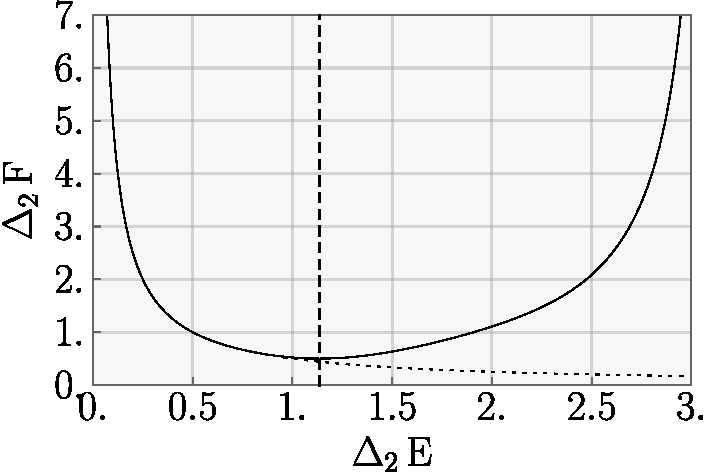
\includegraphics[width=0.8\textwidth]{box-ur2}  
  \caption{The uncertainty region for the particle in a box system, showing the curve obtained from the least eigenvalues of the operators $H_\alpha$ (solid curve), this is the exact boundary curve on the right hand side of the vertical line at $\sqrt{\frac{\pi^2}{3} -2}$ (dashed). On the left hand side the true curve lies between the solid curve and the boundary of the free particle uncertainty region (dotted).}
  \label{fig:box-ur}
  \end{subfigure}
  \begin{subfigure}{\textwidth}
    \centering
    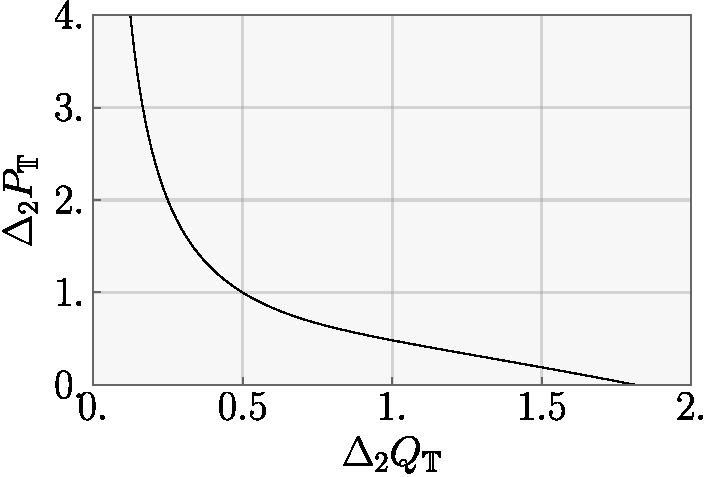
\includegraphics[width=0.8\textwidth]{ring-ur2}  
    \caption{The uncertainty region for the particle on a ring system. Note that this is identical to the top left panel of figure~1 in ref.~\cite{sharp-ur-num-angle}, and is included here only for comparison with figure~\ref{fig:box-ur}.}
    \label{fig:ring-ur}
  \end{subfigure}
  \caption{The box, free particle and ring uncertainty regions.}
\end{figure}
